\documentclass[17pt,a4paper,landscape]{extarticle}
\usepackage[margin=2.35cm,top=0.12cm,left=1.05cm]{geometry}
\usepackage{amsmath}
\usepackage{amssymb}
\usepackage{tasks}
\usepackage{tikz}
\usepackage{xcolor}
\usepackage[sfdefault,lf]{FiraSans}
\renewcommand{\familydefault}{\sfdefault}
\setlength{\parindent}{0pt}
\pagestyle{empty}
\settasks{label=\textbf{\arabic*.}, label-width=2.2em, item-indent=2.95em, column-sep=2.1cm, after-item-skip=9.8em}
\renewcommand{\arraystretch}{1.15}
\everymath{\displaystyle}

\begin{document}
\sffamily
\boldmath

\boldmath

{\LARGE \textbf{Drawing straight-line from given equation — Excellence}}\\[0.2em]
Rearrange to the form $y=mx+c$ when needed, then draw the line carefully.

\begin{tasks}(4)
\task {Draw \mbox{$x+y=2$}. \\[0.4em] 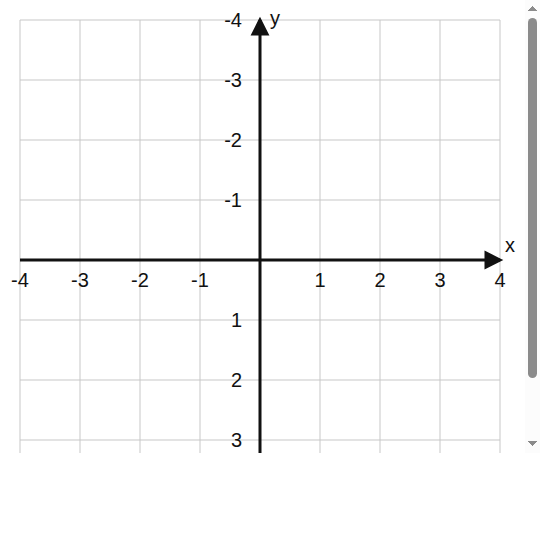
\includegraphics[width=0.88\linewidth]{web-diagrams/coord-grid.png}}
\task {Draw \mbox{$2x+y=-1$}. \\[0.4em] 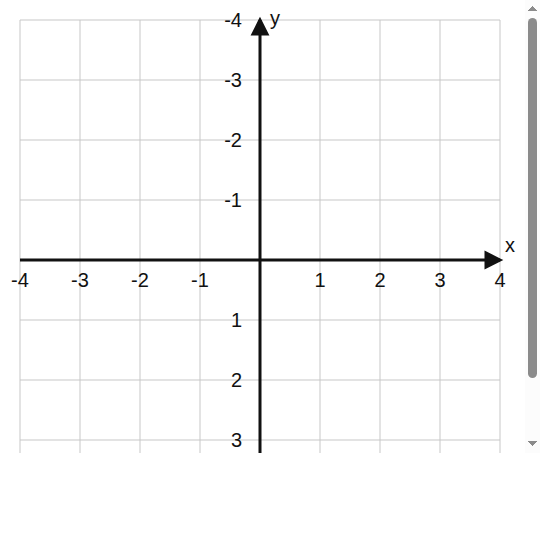
\includegraphics[width=0.88\linewidth]{web-diagrams/coord-grid.png}}
\task {Draw \mbox{$2y-3x=4$}. \\[0.4em] 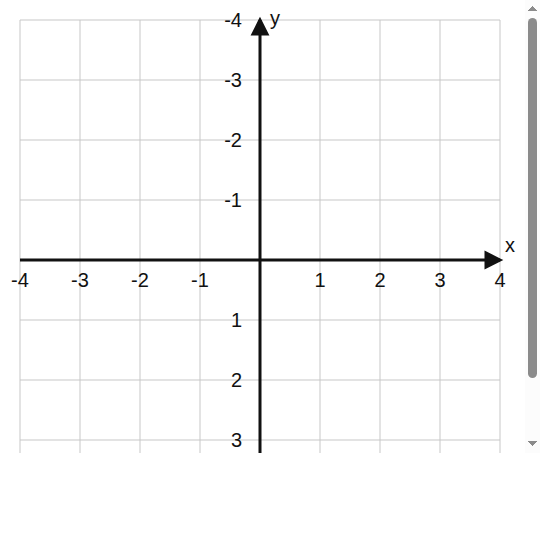
\includegraphics[width=0.88\linewidth]{web-diagrams/coord-grid.png}}
\task {Draw \mbox{$3y+2x=6$}. \\[0.4em] 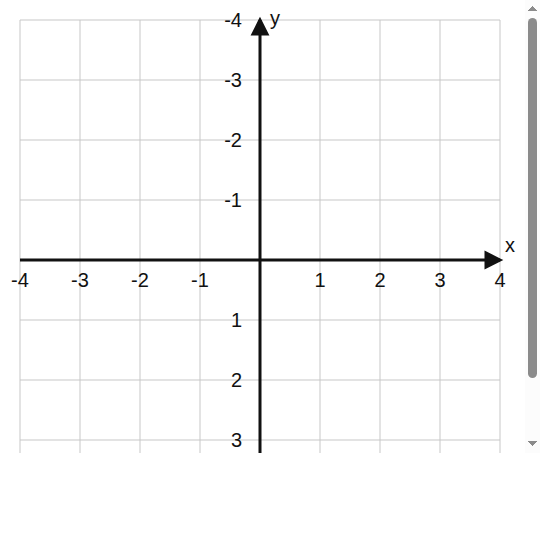
\includegraphics[width=0.88\linewidth]{web-diagrams/coord-grid.png}}
\task {Draw \mbox{$4y=2x-8$}. \\[0.4em] 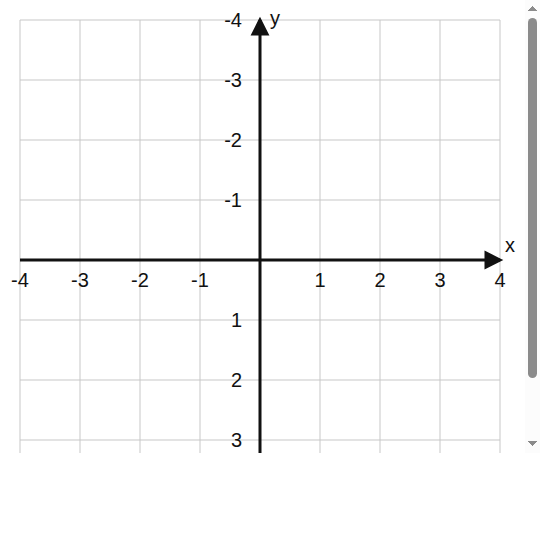
\includegraphics[width=0.88\linewidth]{web-diagrams/coord-grid.png}}
\task {Draw \mbox{$4y=-2x+4$}. \\[0.4em] 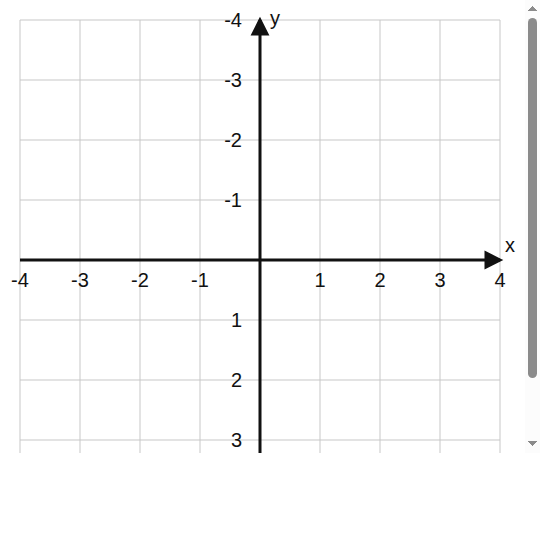
\includegraphics[width=0.88\linewidth]{web-diagrams/coord-grid.png}}
\task {Draw \mbox{$y=\frac{5}{2}x-3$}. \\[0.4em] 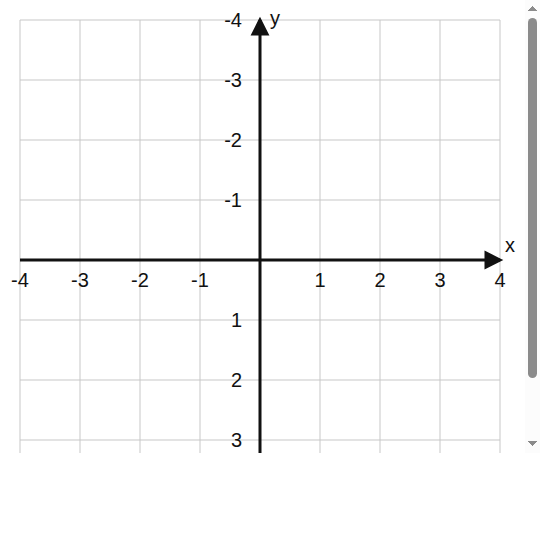
\includegraphics[width=0.88\linewidth]{web-diagrams/coord-grid.png}}
\task {Draw \mbox{$y=-\frac{5}{2}x+4$}. \\[0.4em] 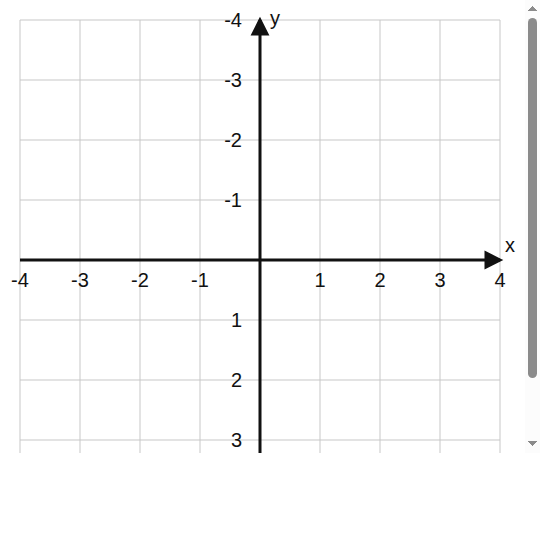
\includegraphics[width=0.88\linewidth]{web-diagrams/coord-grid.png}}
\task {Draw \mbox{$y-3=\frac{3}{2}(x-2)$}. \\[0.4em] 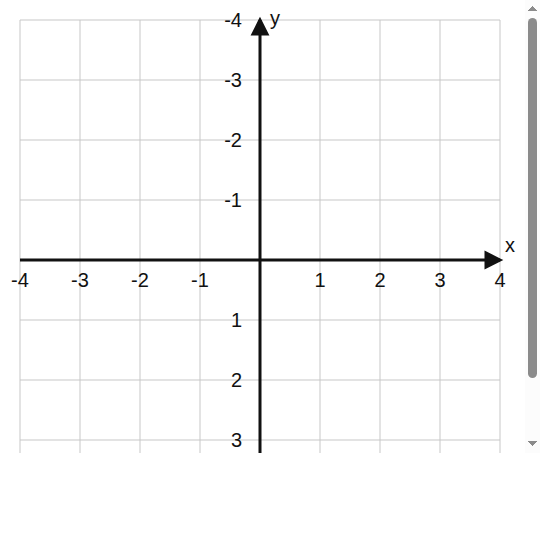
\includegraphics[width=0.88\linewidth]{web-diagrams/coord-grid.png}}
\task {Draw \mbox{$y+1=-\frac{3}{2}(x-1)$}. \\[0.4em] 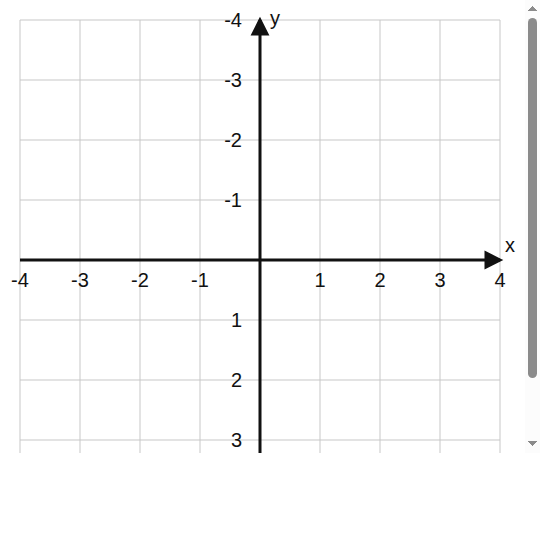
\includegraphics[width=0.88\linewidth]{web-diagrams/coord-grid.png}}
\task {Draw \mbox{$2(y-1)=x+2$}. \\[0.4em] 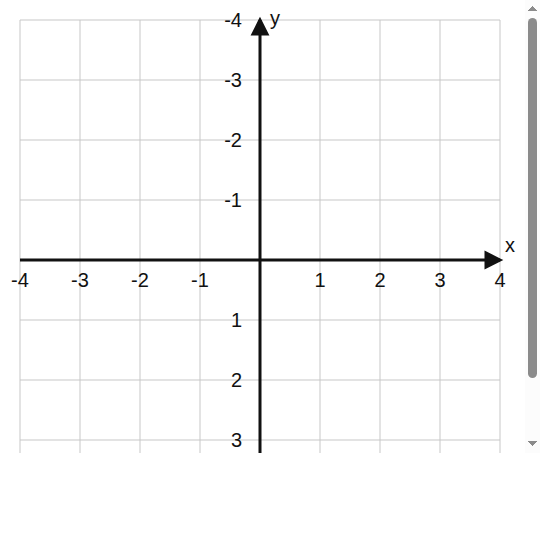
\includegraphics[width=0.88\linewidth]{web-diagrams/coord-grid.png}}
\task {Draw \mbox{$2(y+2)=-x+4$}. \\[0.4em] 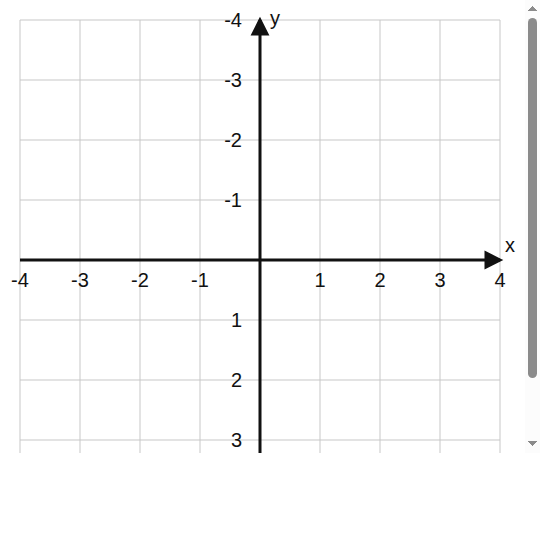
\includegraphics[width=0.88\linewidth]{web-diagrams/coord-grid.png}}
\end{tasks}

\end{document}
